% 正文图8在前，第四问场加密证据可放附录；主文档需加载graphicx、amsmath。
\begin{figure}[htbp]
  \centering
  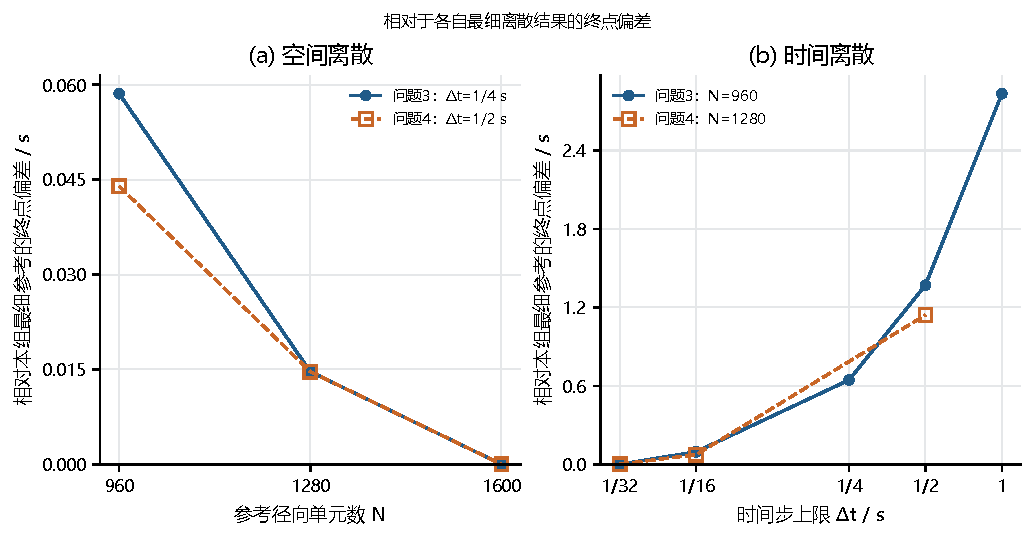
\includegraphics[width=0.98\linewidth]{q4/figures/fig8_combined_convergence.pdf}
  \caption{问题3与问题4的空间、时间离散对干燥终点的影响。纵轴为各模型相对本序列最细参考档的终点绝对偏差，采用线性轴；零点为参考档自比较，并非解析真解误差。空间序列分别固定$\Delta t_3=0.25$ s、$\Delta t_4=0.5$ s，均以本组最大$N$为参考；问题3各网格分别使用自身问题2末态，早期$\tau=1/1024$ s；问题4从初态独立计算，$\tau=1/768$ s。时间序列分别固定$N_3=960$、$N_4=1280$，均以本组最小时间步为参考；问题3共用同一正式问题2末态，问题4保持相同初期步长规则。时间序列事件步长均取$\min(\Delta t_{\max},0.05\ \mathrm{s})$，事件夹逼容差分别为0.01 s与0.01 s。空间含水率差仍需独立验收，不能仅凭本图的终点偏差接受网格。}
  \label{fig:combined-convergence}
\end{figure}

各模型、各序列分别定义
\[E_t^{(q)}=\left|t_+^{(q)}-t_{\mathrm{ref}}^{(q)}\right|,\qquad q=3,4.\]
参考终点是对应离散序列的最细已计算结果，不是解析真解。局部事件括区、终点加密差与场量加密差分别核对，不将其合称为严格总误差上界。

% 以下补图可放第四问数值验证附录。
\begin{figure}[htbp]
  \centering
  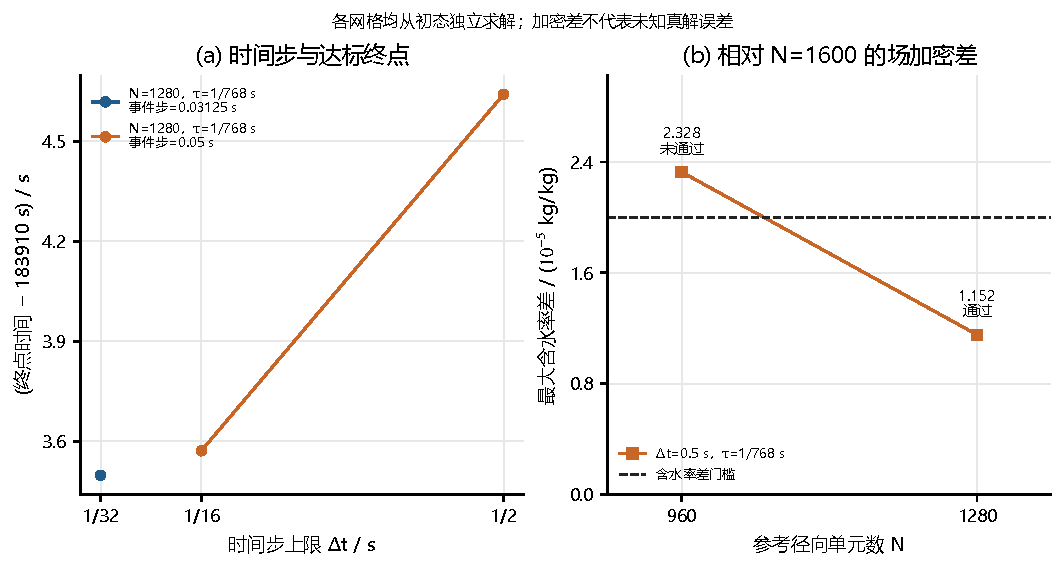
\includegraphics[width=0.98\linewidth]{validation/figures/q4_convergence.pdf}
  \caption{第四问的时间步与场量加密检查。左图为实际时间步下的终点变化；右图为各网格相对更细参考网格的四类含水率最大差，虚线为$2\times10^{-5}$ kg/kg门槛。该补图保留未通过的960网格筛选记录，避免仅以终点差判断网格充分性。}
  \label{fig:q4-convergence}
\end{figure}
